\documentclass[12pt,letterpaper]{exam}
\usepackage[lmargin=1in,rmargin=1in,tmargin=1in,bmargin=1in]{geometry}
\usepackage{../style/exams}

% -------------------
% Course & Exam Information
% -------------------
\newcommand{\course}{MAT 101: Exam 2}
\newcommand{\term}{Fall -- 2021}
\newcommand{\examdate}{12/16/2021}
\newcommand{\timelimit}{85 Minutes}

\setbool{hideans}{false} % Student: True; Instructor: False

% -------------------
% Content
% -------------------
\begin{document}

\examtitle
\instructions{Write your name on the appropriate line on the exam cover sheet. This exam contains \numpages\ pages (including this cover page) and \numquestions\ questions. Check that you have every page of the exam. Answer the questions in the spaces provided on the question sheets. Be sure to answer every part of each question and show all your work.} 
\scores
\bottomline
\newpage

% ---------
% Questions
% ---------
\begin{questions}

% Question 1
\newpage
\question[5] Sketch the quadratic function $f(x)= 5 - 2(x + 1)^2$ in the graph below. Your sketch should include the vertex and axis of symmetry for $f(x)$. 
	\[
	\fbox{
	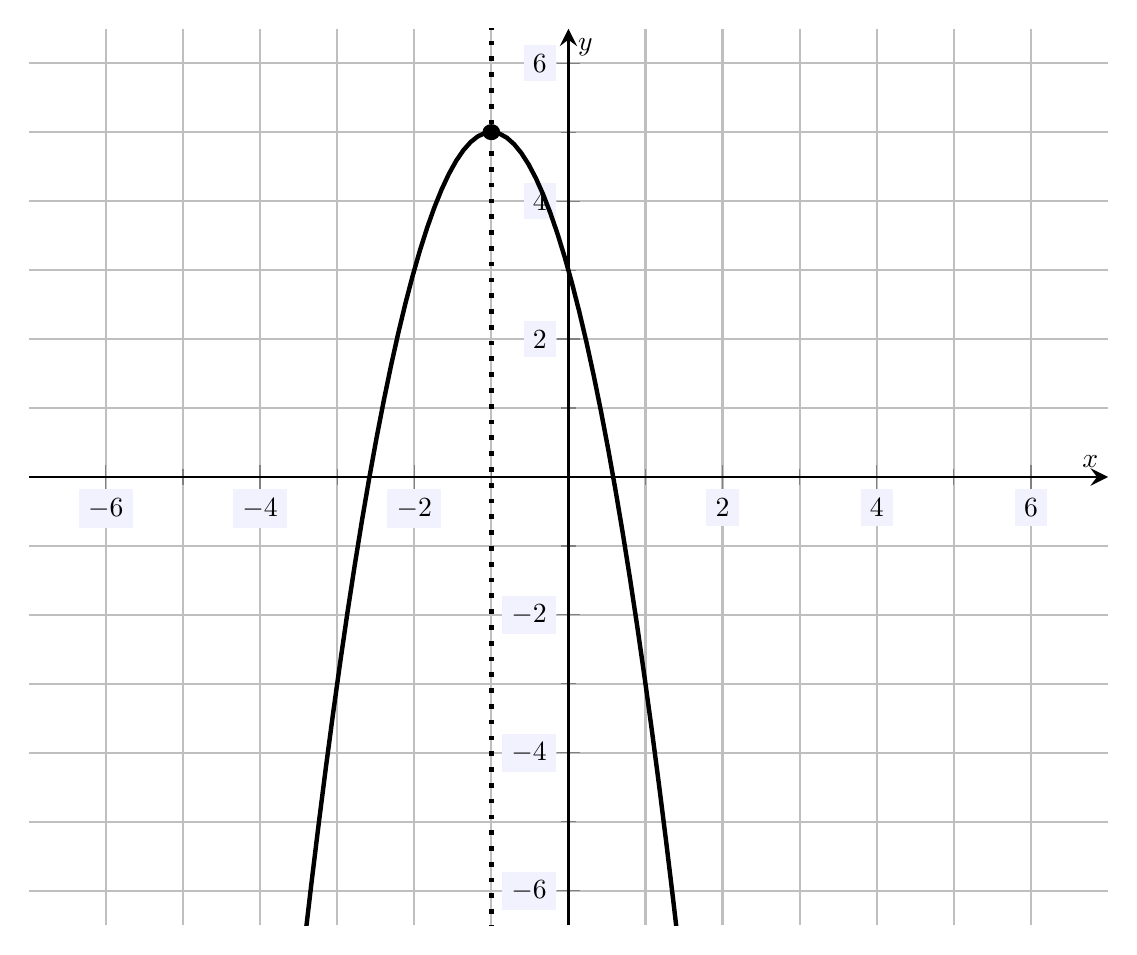
\begin{tikzpicture}[scale=2,every node/.style={scale=0.5}]
	\begin{axis}[
	grid=both,
	axis lines=middle,
	ticklabel style={fill=blue!5!white},
	xmin= -7, xmax=7,
	ymin= -6.5, ymax=6.5,
	xtick={-6,-4,-2,0,2,4,6},
	ytick={-6,-4,-2,0,2,4,6},
	minor tick = {-5,-3,...,5},
	xlabel=\(x\),ylabel=\(y\),
	]
	\addplot[thick, domain= -7:7,samples=150] {5 - 2*(x + 1)^2};
	\draw[dotted,line width= 0.03cm] (-1,-10) -- (-1,10);
	\draw[fill=black] (-1,5) circle (0.1);
	\end{axis}
	\end{tikzpicture}
	}
	\] \pspace

{\noindent\itshape From the form of the function $f(x)= 5 - 2(x + 1)^2$, we can immediately see that the vertex is $(-1, 5)$ and that the parabola opens downwards.}





% Question 2
\newpage
\question[10] Let $f(x)$ be the quadratic function $f(x)= x^2 + 4x + 9$.
\begin{enumerate}[(a)]
\item Find the vertex and axis of symmetry for $f(x)$.
\item Does this parabola open upwards or downwards? Explain.
\item Is the function convex or concave? 
\item Does the function have a maximum or minimum value? Explain. 
\item Find the maximum or minimum value from (d). 
\end{enumerate} \pspace

{\noindent\bfseries Solution.}
\begin{enumerate}[(a)]
{\itshape
\item We know that the $x$-coordinate of the vertex is\dots
	\[
	x= \dfrac{-b}{2a}= \dfrac{-4}{2(1)}= \dfrac{-4}{2}= -2
	\]
The $y$-coordinate of the vertex is $f(-2)= (-2)^2 + 4(-2) + 9= 4 - 8 + 9= 5$. Therefore, the vertex is $(-2, 5)$. It is also immediate that the axis of symmetry is $x= -2$. 
	
	\[
	\boxed{%
	\begin{aligned}
	\text{Vertex: }& (-2, 5) \\
	\text{Axis of Symmetry: }& x= -2
	\end{aligned}
	}
	\] \pspace

\item Because $a= 1 > 0$, the parabola opens upwards. \pspace

\item Because the parabola opens upwards, the function is convex. \pspace

\item Because the parabola opens upwards, the function has a minimum. \pspace

\item We know the minimum value occurs at the vertex. The vertex has coordinate $(-2, 5)$. Therefore, the minimum value is $5$. 
}
\end{enumerate}





% Question 3
\newpage
\question[5] Find the vertex form of $y= 3x^2 - 6x + 10$. \pspace

{\noindent\itshape We complete the square. First, we factor out a $3$ to obtain $y= 3(x^2 - 2x + \frac{10}{3})$. Observe that $\frac{1}{2} \cdot -2= -1$ and that $(-1)^2= 1$. Then\dots
	\[
	\begin{aligned}
	y&= 3x^2 - 6x + 10 \\[0.3cm]
	y&= 3 \left( x^2 - 2x + \dfrac{10}{3} \right) \\[0.3cm]
	y&= 3 \left( x^2 - 2x + 1 - 1 + \frac{10}{3} \right) \\[0.3cm]
	y&= 3 \left( (x - 1)^2 + \dfrac{7}{3} \right) \\[0.3cm]
	y&= 3(x - 1)^2 + 7
	\end{aligned}
	\] \pspace
	
	\[
	\boxed{y= 3(x - 1)^2 + 7}
	\]
}





% Question 4
\newpage
\question[5] Factor the polynomial $x^2 - 8x - 33$. \pspace

	\begin{table}[!ht]
	\centering
	\underline{\bfseries 33} \pvspace{0.2cm}
	\begin{tabular}{rr}
	$1 \cdot -33$ & $-32$ \\
	$-1 \cdot 33$ & $32$ \\ \hline
	\multicolumn{1}{|r}{$3 \cdot -11$} & \multicolumn{1}{r|}{$-8$} \\ \hline
	$-3 \cdot 11$ & $8$ \\
	\end{tabular}
	\end{table}

	\[
	x^2 - 8x - 33= (x - 11)(x + 3)
	\] \pspace
	
	\[
	\boxed{(x - 11)(x + 3)}
	\]





% Question 5
\newpage
\question[5] Factor the polynomial $2x^2 + 11x + 15$. \pspace

	\[
	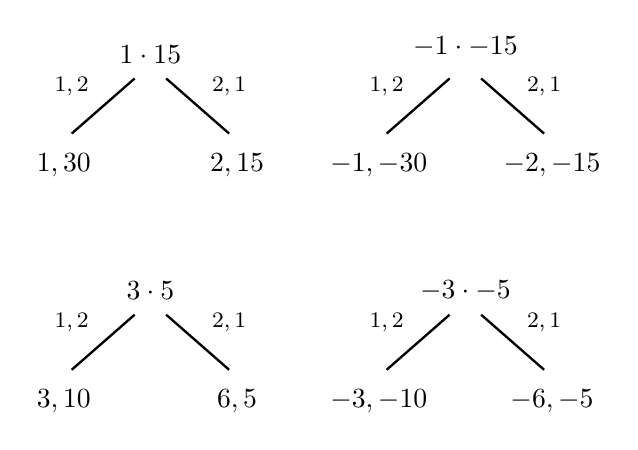
\begin{tikzpicture}
	\node at (0,0) {$1 \cdot 15$};
	\node at (-1.0,-0.4) {\footnotesize$1, 2$};
	\draw[line width=0.03cm,label={1}] (-0.2,-0.3) -- (-1,-1);
	\node at (-1.1,-1.4) {$1, 30$};
	\node at (1.0,-0.4) {\footnotesize$2, 1$};
	\draw[line width=0.03cm] (0.2,-0.3) -- (1,-1);
	\node at (1.1,-1.4) {$2, 15$};	
	
	\tikzset{shift={(4,0)}}

	\node at (0,0.1) {$-1 \cdot -15$};
	\node at (-1.0,-0.4) {\footnotesize$1, 2$};
	\draw[line width=0.03cm,label={1}] (-0.2,-0.3) -- (-1,-1);
	\node at (-1.1,-1.4) {$-1, -30$};
	\node at (1.0,-0.4) {\footnotesize$2, 1$};
	\draw[line width=0.03cm] (0.2,-0.3) -- (1,-1);
	\node at (1.1,-1.4) {$-2, -15$};
	
	\tikzset{shift={(-4,-3)}}
	
	\node at (0,0) {$3 \cdot 5$};
	\node at (-1.0,-0.4) {\footnotesize$1, 2$};
	\draw[line width=0.03cm,label={1}] (-0.2,-0.3) -- (-1,-1);
	\node at (-1.1,-1.4) {$3, 10$};
	\node at (1.0,-0.4) {\footnotesize$2, 1$};
	\draw[line width=0.03cm] (0.2,-0.3) -- (1,-1);
	\node at (1.1,-1.4) {$6, 5$};
	
	\tikzset{shift={(4,0)}}

	\node at (0,0) {$-3 \cdot -5$};
	\node at (-1.0,-0.4) {\footnotesize$1, 2$};
	\draw[line width=0.03cm,label={1}] (-0.2,-0.3) -- (-1,-1);
	\node at (-1.1,-1.4) {$-3, -10$};
	\node at (1.0,-0.4) {\footnotesize$2, 1$};
	\draw[line width=0.03cm] (0.2,-0.3) -- (1,-1);
	\node at (1.1,-1.4) {$-6, -5$};
	\end{tikzpicture}
	\]

	\[
	2x^2 + 11x + 15= (2x + 5)(x + 3)
	\] \pspace
	
	\[
	\boxed{(2x + 5)(x + 3)}
	\]





% Question 6
\newpage
\question[5] Consider the function $f(x)= x^2 + 6x - 40$. Find the $x$ and $y$ intercepts for this function. \pspace

{\noindent\itshape The $y$-intercept occurs when $x= 0$. But then $y= f(0)= 0^2 + 6(0) - 40= 0 + 0 - 40= -40$. Therefore, the $y$-intercept is $(0, -40)$. \pspace

The $x$-intercepts occur when $y= 0$. But then $x^2 + 6x - 40= 0$. Observe\dots
	\[
	\begin{aligned}
	x^2 + 6x - 40&= 0 \\
	(x - 4)(x + 10)&= 0
	\end{aligned}
	\]
But then either $x - 4= 0$, i.e. $x= 4$, or $x + 10= 0$, i.e. $x= -10$. Therefore, the $x$-intercepts are $(4, 0)$ and $(-10, 0)$. \pvspace{1cm}
	\[
	\boxed{%
	\begin{aligned}
	y\text{-intercept: }& (0, -40) \\
	x\text{-intercepts: }& (-10, 0), (4, 0)
	\end{aligned}
	}
	\]
}





% Question 7
\newpage
\question[5] Find the solutions to $x^2= 8x - 16$. \pspace

	\[
	\begin{aligned}
	x^2&= 8x - 16 \\[0.3cm]
	x^2 - 8x + 16&= 0 \\[0.3cm]
	(x - 4)^2&= 0 \\[0.3cm]
	x - 4&= 0 \\[0.3cm]
	x&= 4
	\end{aligned}
	\] \pspace
	
	\[
	\boxed{x= 4}
	\]





% Question 8
\newpage
\question[5] Using the quadratic equation, find the solutions to $3 - 2x^2= 6x$. \pspace

{\itshape First, we re-arrange the equation:
	\[
	\begin{aligned}
	3 - 2x^2&= 6x \\
	2x^2 + 6x - 3&= 0 
	\end{aligned}
	\]
Now we apply the quadratic equation:
	\[
	\begin{aligned}
	x&= \dfrac{-b \pm \sqrt{b^2 - 4ac}}{2a} \\[0.3cm]
	x&= \dfrac{-6 \pm \sqrt{6^2 - 4(2)(-3)}}{2(2)} \\[0.3cm]
	x&= \dfrac{-6 \pm \sqrt{36 + 24}}{4} \\[0.3cm]
	x&= \dfrac{-6 \pm \sqrt{60}}{4} \\[0.3cm]
	x&= \dfrac{-6 \pm \sqrt{4 \cdot 15}}{4} \\[0.3cm]
	x&= \dfrac{-6 \pm 2\sqrt{15}}{4} \\[0.3cm]
	x&= \dfrac{-3 \pm \sqrt{15}}{2}
	\end{aligned}
	\] \pspace
	
	\[
	\boxed{x= \dfrac{-3 - \sqrt{15}}{2},\enskip \dfrac{-3 + \sqrt{15}}{2}}
	\]
}





% Question 9
\newpage
\question[10] Consider the rational function $f(x)= \dfrac{x^2 - 25}{x^2 - x - 20}$. 
\begin{enumerate}[(a)]
\item Find the domain for $f(x)$. 
\item Find the vertical asymptotes for $f(x)$. 
\item Find the zeros for $f(x)$. 
\end{enumerate} \pspace

{\noindent\bfseries Solution.}

	\[
	f(x)= \dfrac{x^2 - 25}{x^2 - x - 20}= \dfrac{(x - 5)(x + 5)}{(x - 5)(x + 4)}
	\] \pspace

\begin{enumerate}[(a)]
{\itshape
\item The domain of a rational function consists of the real numbers for which the denominator is not zero. If the denominator were zero, then $(x - 5)(x + 4)= 0$. But then either $x - 5= 0$, i.e. $x= 5$, or $x + 4= 0$, i.e. $x= -4$. Therefore, the domain is the set of real numbers such that $x \neq 5, -4$. 
	\[
	\boxed{%
	x \in \mathbb{R} \text{ such that } x \neq -4, 5
	}
	\] \pspace

\item We see that for $x \neq -4, 5$, 
	\[
	f(x)= \dfrac{x^2 - 25}{x^2 - x - 20}= \dfrac{(x - 5)(x + 5)}{(x - 5)(x + 4)}= \dfrac{\cancel{(x - 5)}(x + 5)}{\cancel{(x - 5)}(x + 4)}= \dfrac{x + 5}{x + 4}
	\]
The vertical asymptotes for $f(x)$ will be where the denominator vanishes in this reduced function. But then $x + 4= 0$, i.e. $x= -4$. Therefore, the only vertical asymptote is $x= -4$. 
	\[
	\boxed{%
	x= -4
	}
	\] \pspace

\item We see that for $x \neq -4, 5$, 
	\[
	f(x)= \dfrac{x^2 - 25}{x^2 - x - 20}= \dfrac{(x - 5)(x + 5)}{(x - 5)(x + 4)}= \dfrac{\cancel{(x - 5)}(x + 5)}{\cancel{(x - 5)}(x + 4)}= \dfrac{x + 5}{x + 4}
	\]
The zeros for $f(x)$ will be where the numerator vanishes in this reduced function. But then $x + 5= 0$, i.e. $x= -5$. Therefore, the only zero is $x= -5$. 
	\[
	\boxed{%
	x= -5
	}
	\] \pspace
}
\end{enumerate}





% Question 10
\newpage
\question[5] Compute the following, being sure to simplify as much as possible: 
	\[
	\dfrac{x + 2}{x^2 - 1} - \dfrac{4}{x^2 + 4x + 3}
	\] \pspace

	\[
	\begin{aligned}
	\dfrac{x + 2}{x^2 - 1} - \dfrac{4}{x^2 + 4x + 3}&= \dfrac{x + 2}{(x - 1)(x + 1)} - \dfrac{4}{(x + 1)(x + 3)} \\[0.3cm]
	&= \dfrac{(x + 2)(x + 3)}{(x - 1)(x + 1)(x + 3)} - \dfrac{4(x - 1)}{(x + 1)(x + 3)(x -1)} \\[0.3cm]
	&= \dfrac{(x + 2)(x + 3) - 4(x - 1)}{(x - 1)(x + 1)(x + 3)} \\[0.3cm]
	&= \dfrac{(x^2 + 3x + 2x + 6) - (4x - 4)}{(x - 1)(x + 1)(x + 3)} \\[0.3cm]
	&= \dfrac{x^2 + 5x + 6 - 4x + 4}{(x - 1)(x + 1)(x + 3)} \\[0.3cm]
	&= \dfrac{x^2 + x + 10}{(x - 1)(x + 1)(x + 3)}
	\end{aligned}
	\] \pspace
	
	\[
	\boxed{\dfrac{x^2 + x + 10}{(x - 1)(x + 1)(x + 3)}}
	\]





% Question 11
\newpage
\question[5] Compute the following, begin sure to simplify as much as possible:
	\[
	\dfrac{\phantom{--}\dfrac{x^2 - 4x}{x^2 - 9}\phantom{--}}{\dfrac{x^2 + 2x - 24}{x^2 + 10x + 21}}
	\] \pspace

	\[
	\begin{aligned}
	\dfrac{\phantom{--}\dfrac{x^2 - 4x}{x^2 - 9}\phantom{--}}{\dfrac{x^2 + 2x - 24}{x^2 + 10x + 21}}&= \dfrac{x^2 - 4x}{x^2 - 9} \cdot \dfrac{x^2 + 10x + 21}{x^2 + 2x - 24} \\[0.3cm]
	&= \dfrac{x(x - 4)}{(x - 3)(x + 3)} \cdot \dfrac{(x + 3)(x + 7)}{(x + 6)(x - 4)} \\[0.3cm]
	&= \dfrac{x\cancel{(x - 4)}}{(x - 3)\cancel{(x + 3)}} \cdot \dfrac{\cancel{(x + 3)}(x + 7)}{(x + 6)\cancel{(x - 4)}} \\[0.3cm]
	&= \dfrac{x(x + 7)}{(x - 3)(x + 6)}
	\end{aligned}
	\] \pspace
	
	\[
	\boxed{\dfrac{x(x + 7)}{(x - 3)(x + 6)}}
	\]





% Question 12
\newpage
\question[5] Solve the equation $4^{1 - x} - 3= 13$. \pspace

	\[
	\begin{aligned}
	4^{1 - x} - 3&= 13 \\[0.3cm]
	4^{1 - x}&= 16 \\[0.3cm]
	4^{1 - x}&= 4^2 \\[0.3cm]
	1 - x&= 2 \\[0.3cm]
	x&= -1
	\end{aligned}
	\]
	
	\begin{center} {\bfseries OR} \end{center}
	
	\[
	\begin{aligned}
	4^{1 - x} - 3&= 13 \\[0.3cm]
	4^{1 - x}&= 16 \\[0.3cm]
	\log_4 4^{1 - x}&= \log_4 16 \\[0.3cm]
	1 - x&= 2 \\[0.3cm]
	x&= - 1
	\end{aligned}
	\] \pspace
	
	\[ 
	\boxed{x= -1}
	\]





% Question 13
\newpage
\question[5] Solve the equation $2e^{-x} + 5= 17$. \pspace

	\[
	\begin{aligned}
	2e^{-x} + 5&= 17 \\[0.3cm]
	2e^{-x}&= 12 \\[0.3cm]
	e^{-x}&= 6 \\[0.3cm]
	\ln e^{-x}&= \ln 6 \\[0.3cm]
	-x&= \ln 6 \\[0.3cm]
	x&= -\ln 6
	\end{aligned}
	\] \pspace
	
	\[
	\boxed{x= -\ln 6}
	\]





% Question 14
\newpage
\question[5] Solve the equation $\log_2(x + 5)= 3$. \pspace

	\[
	\begin{aligned}
	\log_2(x + 5)&= 3 \\[0.3cm]
	2^{\log_2(x + 5)}&= 2^3 \\[0.3cm]
	x + 5&= 8 \\[0.3cm]
	x&= 3
	\end{aligned}
	\] \pspace
	
	\[
	\boxed{x= 3}
	\]





% Question 15
\newpage
\question[5] Solve the equation $\log_5(x + 7) + \log_5(x + 3)= 1$. \pspace

{\itshape
	\[
	\begin{aligned}
	\log_5(x + 7) + \log_5(x + 3)&= 1 \\[0.3cm]
	\log_5\big( (x + 7)(x + 3) \big)&= 1 \\[0.3cm]
	5^{\log_5\big( (x + 7)(x + 3) \big)}&= 5^1 \\[0.3cm]
	(x + 7)(x + 3)&= 5 \\[0.3cm]
	x^2 + 10x + 21&= 5 \\[0.3cm]
	x^2 + 10x + 16&= 0 \\[0.3cm]
	(x + 2)(x + 8)&= 0 \\[0.3cm]
	x + 2= 0 \text{ or } x +& 8= 0 \\[0.3cm]
	x= -2 \text{ or } x= &-\!8 
	\end{aligned}
	\] \pspace

However, observe that if $x= -8$, then the left side contains the term $\log_5(-8 + 7)= \log_5(-1)$, which is undefined. Finally, observe that if $x= -2$, we have\dots

	\[
	\log_5(-2 + 7) + \log_5(-2 + 3)= \log_5(5) + \log_5(1)= 1 + 0= 1
	\] \pspace
	
	\[
	\boxed{x= -2}
	\]
}





% Question 16
\newpage
\question[5] Suppose you invest \$500 in an account which gains 8\% annual interest, compounded semiannually. Find an expression which computes the amount of money in the account after 5~years. \pspace

	\[
	\begin{aligned}
	F&= P \left(1 + \dfrac{r}{k} \right)^{kt} \\[0.3cm]
	F&= 500 \left(1 + \dfrac{0.08}{2} \right)^{2 \cdot 5} \\[0.3cm]
	F&= 500 \left(1 + 0.04 \right)^{10} \\[0.3cm]
	F&= 500 (1.04)^{10}
	\end{aligned}
	\] \pspace
	
	\[
	\boxed{500 (1.04)^{10} \approx \$740.12}
	\]





% Question 17
\newpage
\question[5] Solve the following system of equations:
	\[
	\begin{aligned}
	x - y&= 5 \\
	x + y&= 3
	\end{aligned}
	\] \pspace

{\itshape Using substitution, from the first equation, we have\dots
	\[
	\begin{aligned}
	x - y&= 5 \\
	y&= x - 5
	\end{aligned}
	\]
Using this in the second equation, we have\dots
	\[
	\begin{aligned}
	x + y&= 3 \\
	x + (x - 5)&= 3 \\
	x + x - 5&= 3 \\
	2x - 5&= 3 \\
	2x&= 8 \\
	x&= 4
	\end{aligned}
	\]
But then we have $y= x - 5= 4 - 5= -1$. Therefore, the solution is $(4, -1)$. 

	\begin{center} {\bfseries OR} \end{center}

Using elimination, we add the two equations:
	\[
	\begin{aligned}
	x - y&= 5 \\
	x + y&= 3 \\ \hline
	2x&= 8 \\
	x&= 4
	\end{aligned}
	\]
Using this in the first equation, we have\dots
	\[
	\begin{aligned}
	x - y&= 5 \\
	4 - y&= 5 \\
	y&= -1
	\end{aligned}
	\]
Therefore, the solution is $(4, -1)$. \pspace
	\[
	\boxed{(x, y)= (4, -1)}
	\]
}





% Question 18
\newpage
\question[5] Solve the following system of equations:
	\[
	\begin{aligned}
	-3x + 15y&= 9 \\
	2x + 5y&= -3
	\end{aligned}
	\] \pspace

{\itshape Using substitution, from the first equation, we have\dots
	\[
	\begin{aligned}
	-3x + 15y&= 9 \\
	15y&= 3x + 9 \\
	y&= \frac{1}{5}\,x + \frac{3}{5}
	\end{aligned}
	\]
Using this in the second equation, we have\dots
	\[
	\begin{aligned}
	2x + 5y&= -3 \\
	2x + 5 \left( \frac{1}{5}\,x + \frac{3}{5} \right)&= -3 \\
	2x + x + 3&= -3 \\
	3x + 3&= -3 \\
	3x&= -6 \\
	x&= -2
	\end{aligned}
	\]
Then we have $y= \frac{1}{5}\, x + \frac{3}{5}= \frac{1}{5} \cdot -2 + \frac{3}{5}= -\frac{2}{5} + \frac{3}{5}= \frac{1}{5}$. Therefore, the solution is $(-2, \frac{1}{5})$. 

	\begin{center} {\bfseries OR} \end{center}

Using elimination, we multiply the second equation by $-3$. This yields\dots
	\[
	\begin{aligned}
	-3x + 15y&= 9 \\
	-6x - 15y&= 9
	\end{aligned}
	\]
Adding these equations, we have\dots
	\[
	\begin{aligned}
	-3x + 15y&= 9 \\
	-6x - 15y&= 9 \\ \hline
	-9x&= 18 \\
	x&= -2
	\end{aligned}
	\]
Using this in the second equation, we have $2(-2) + 5y= -3$ so that $5y - 4= -3$. But then $5y= 1$. Therefore, $y= \frac{1}{5}$. The solution is then $(-2, \frac{1}{5})$. \pspace

	\[
	\boxed{(x, y)= \left( -2,\; \frac{1}{5} \right)}
	\]
}


\end{questions}
\end{document}